\documentclass{standalone}
\usepackage{tikz}
\usetikzlibrary{patterns, positioning}
\usepackage[sfdefault]{ClearSans} %% option 'sfdefault' activates Clear Sans as the default text font
\usepackage[T1]{fontenc}

\begin{document}
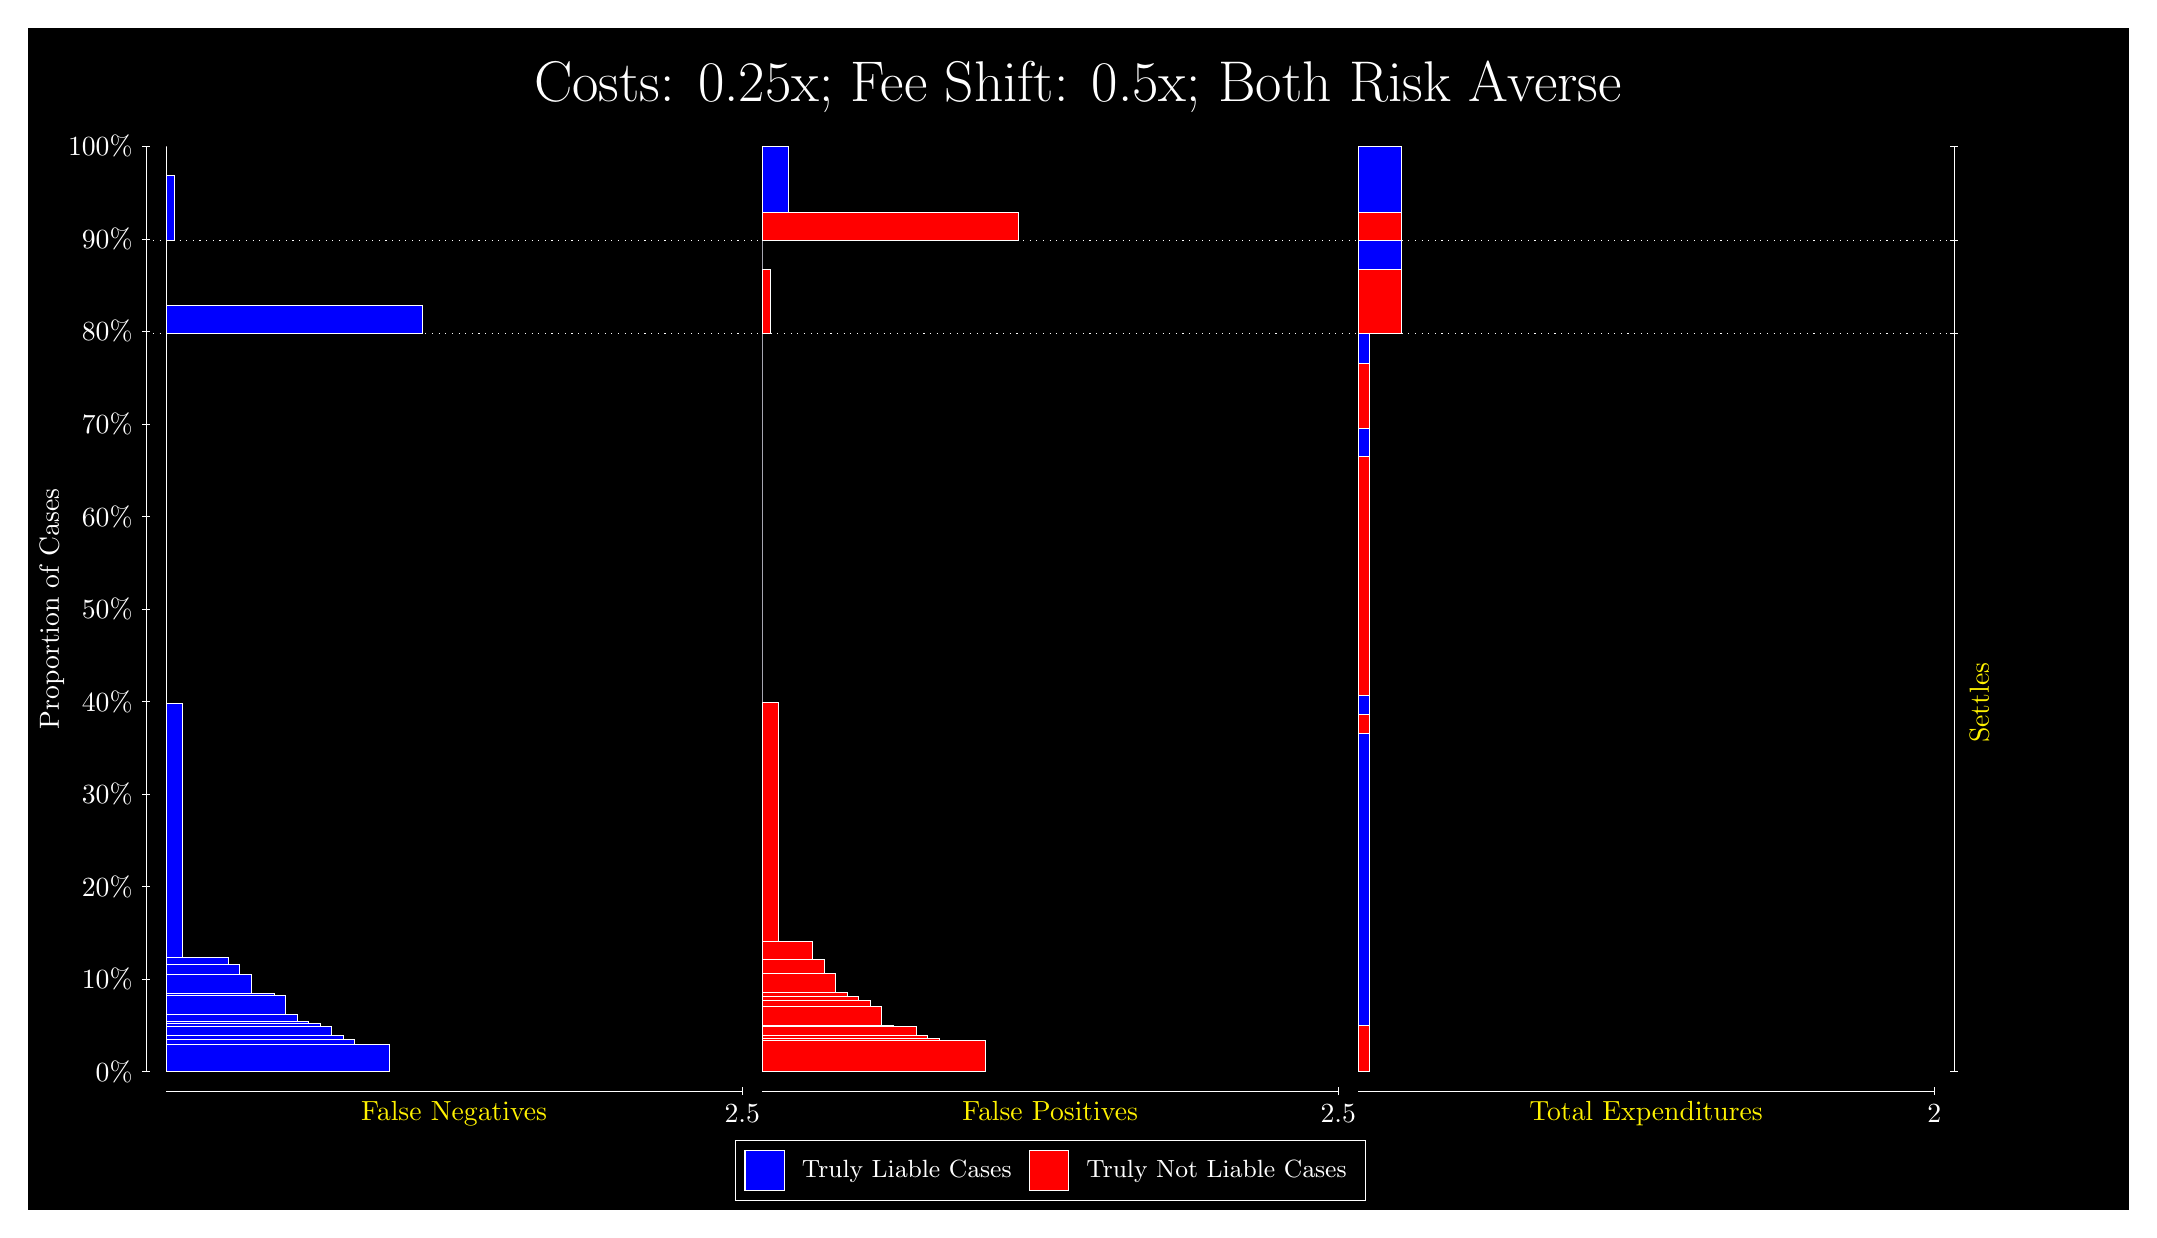
\begin{tikzpicture}
\draw[fill=black] (0,0) rectangle (26.667,15);
\draw[text=white] (0,13.5) rectangle (26.667,15) node[midway] {\huge Costs: 0.25x; Fee Shift: 0.5x; Both Risk Averse};
\draw[white, very thin] (1.5,1.75) -- (1.5,13.5);
\node[rotate=90, text=white, anchor=center] at (0.3, 7.625) {Proportion of Cases};
\draw[white, very thin] (1.45,1.75) -- (1.55,1.75);
\node[text=white, anchor=east] at (1.45, 1.75) {0\%};
\draw[white, very thin] (1.45,2.925) -- (1.55,2.925);
\node[text=white, anchor=east] at (1.45, 2.925) {10\%};
\draw[white, very thin] (1.45,4.1) -- (1.55,4.1);
\node[text=white, anchor=east] at (1.45, 4.1) {20\%};
\draw[white, very thin] (1.45,5.275) -- (1.55,5.275);
\node[text=white, anchor=east] at (1.45, 5.275) {30\%};
\draw[white, very thin] (1.45,6.45) -- (1.55,6.45);
\node[text=white, anchor=east] at (1.45, 6.45) {40\%};
\draw[white, very thin] (1.45,7.625) -- (1.55,7.625);
\node[text=white, anchor=east] at (1.45, 7.625) {50\%};
\draw[white, very thin] (1.45,8.8) -- (1.55,8.8);
\node[text=white, anchor=east] at (1.45, 8.8) {60\%};
\draw[white, very thin] (1.45,9.975) -- (1.55,9.975);
\node[text=white, anchor=east] at (1.45, 9.975) {70\%};
\draw[white, very thin] (1.45,11.15) -- (1.55,11.15);
\node[text=white, anchor=east] at (1.45, 11.15) {80\%};
\draw[white, very thin] (1.45,12.325) -- (1.55,12.325);
\node[text=white, anchor=east] at (1.45, 12.325) {90\%};
\draw[white, very thin] (1.45,13.5) -- (1.55,13.5);
\node[text=white, anchor=east] at (1.45, 13.5) {100\%};

\draw[white, very thin] (24.457,1.75) -- (24.457,13.5);
\draw[white, very thin] (24.407,1.75) -- (24.507,1.75);
\node[anchor=west] at (24.407, 1.75) {};
\draw[white, very thin] (24.407,11.12) -- (24.507,11.12);
\node[anchor=west] at (24.407, 11.12) {};
\draw[white, very thin] (24.407,12.303) -- (24.507,12.303);
\node[anchor=west] at (24.407, 12.303) {};
\draw[white, very thin] (24.407,13.5) -- (24.507,13.5);
\node[anchor=west] at (24.407, 13.5) {};

\draw[white, very thin, fill=blue] (1.75,1.75) rectangle (4.5861,2.0959);
\draw[white, very thin, fill=blue] (1.75,2.0959) rectangle (4.1469,2.1616);
\draw[white, very thin, fill=blue] (1.75,2.1616) rectangle (4.0006,2.2136);
\draw[white, very thin, fill=blue] (1.75,2.2136) rectangle (3.8542,2.3194);
\draw[white, very thin, fill=blue] (1.75,2.3194) rectangle (3.7078,2.3566);
\draw[white, very thin, fill=blue] (1.75,2.3566) rectangle (3.5614,2.3862);
\draw[white, very thin, fill=blue] (1.75,2.3862) rectangle (3.415,2.4716);
\draw[white, very thin, fill=blue] (1.75,2.4716) rectangle (3.2687,2.7203);
\draw[white, very thin, fill=blue] (1.75,2.7203) rectangle (3.1223,2.7438);
\draw[white, very thin, fill=blue] (1.75,2.7438) rectangle (2.8295,2.9828);
\draw[white, very thin, fill=blue] (1.75,2.9828) rectangle (2.6832,3.1066);
\draw[white, very thin, fill=blue] (1.75,3.1066) rectangle (2.5368,3.2041);
\draw[white, very thin, fill=blue] (1.75,3.2041) rectangle (1.9513,6.4276);
\draw[white, very thin, fill=red] (1.75,6.4276) rectangle (1.75,11.12);
\draw[white, very thin, fill=blue] (1.75,11.12) rectangle (5.0069,11.484);
\draw[white, very thin, fill=red] (1.75,11.484) rectangle (1.75,12.303);
\draw[white, very thin, fill=blue] (1.75,12.303) rectangle (1.8598,13.136);
\draw[white, very thin, fill=red] (1.75,13.136) rectangle (1.75,13.5);
\draw[white, very thin, fill=red] (9.3189,1.75) rectangle (12.155,2.1488);
\draw[white, very thin, fill=red] (9.3189,2.1488) rectangle (11.569,2.1768);
\draw[white, very thin, fill=red] (9.3189,2.1768) rectangle (11.423,2.2125);
\draw[white, very thin, fill=red] (9.3189,2.2125) rectangle (11.277,2.3194);
\draw[white, very thin, fill=red] (9.3189,2.3194) rectangle (10.984,2.3351);
\draw[white, very thin, fill=red] (9.3189,2.3351) rectangle (10.838,2.5739);
\draw[white, very thin, fill=red] (9.3189,2.5739) rectangle (10.691,2.6593);
\draw[white, very thin, fill=red] (9.3189,2.6593) rectangle (10.545,2.7031);
\draw[white, very thin, fill=red] (9.3189,2.7031) rectangle (10.398,2.7586);
\draw[white, very thin, fill=red] (9.3189,2.7586) rectangle (10.252,2.995);
\draw[white, very thin, fill=red] (9.3189,2.995) rectangle (10.106,3.1743);
\draw[white, very thin, fill=red] (9.3189,3.1743) rectangle (9.9593,3.4028);
\draw[white, very thin, fill=red] (9.3189,3.4028) rectangle (9.5201,6.4427);
\draw[white, very thin, fill=blue] (9.3189,6.4427) rectangle (9.3189,11.12);
\draw[white, very thin, fill=red] (9.3189,11.12) rectangle (9.4287,11.939);
\draw[white, very thin, fill=blue] (9.3189,11.939) rectangle (9.3189,12.303);
\draw[white, very thin, fill=red] (9.3189,12.303) rectangle (12.576,12.667);
\draw[white, very thin, fill=blue] (9.3189,12.667) rectangle (9.6482,13.5);
\draw[white, very thin, fill=red] (16.888,1.75) rectangle (17.025,2.3351);
\draw[white, very thin, fill=blue] (16.888,2.3351) rectangle (17.025,6.0423);
\draw[white, very thin, fill=red] (16.888,6.0423) rectangle (17.025,6.2812);
\draw[white, very thin, fill=blue] (16.888,6.2812) rectangle (17.025,6.5299);
\draw[white, very thin, fill=red] (16.888,6.5299) rectangle (17.025,9.5698);
\draw[white, very thin, fill=blue] (16.888,9.5698) rectangle (17.025,9.9156);
\draw[white, very thin, fill=red] (16.888,9.9156) rectangle (17.025,10.745);
\draw[white, very thin, fill=blue] (16.888,10.745) rectangle (17.025,11.12);
\draw[white, very thin, fill=red] (16.888,11.12) rectangle (17.437,11.939);
\draw[white, very thin, fill=blue] (16.888,11.939) rectangle (17.437,12.303);
\draw[white, very thin, fill=red] (16.888,12.303) rectangle (17.437,12.667);
\draw[white, very thin, fill=blue] (16.888,12.667) rectangle (17.437,13.5);
\draw[white, dotted] (1.5,11.12) -- (24.457,11.12);
\draw[white, dotted] (1.5,12.303) -- (24.457,12.303);
\draw[white, very thin] (1.75,1.5) -- (9.0689,1.5);
\node[text=yellow, anchor=north] at (5.4094, 1.5) {False Negatives};
\draw[white, very thin] (9.0689,1.45) -- (9.0689,1.55);
\node[text=white, anchor=north] at (9.0689, 1.45) {2.5};

\draw[white, very thin] (9.3189,1.5) -- (16.638,1.5);
\node[text=yellow, anchor=north] at (12.978, 1.5) {False Positives};
\draw[white, very thin] (16.638,1.45) -- (16.638,1.55);
\node[text=white, anchor=north] at (16.638, 1.45) {2.5};

\draw[white, very thin] (16.888,1.5) -- (24.207,1.5);
\node[text=yellow, anchor=north] at (20.547, 1.5) {Total Expenditures};
\draw[white, very thin] (24.207,1.45) -- (24.207,1.55);
\node[text=white, anchor=north] at (24.207, 1.45) {2};

\node[text=yellow, centered, rotate=90] at (24.777, 6.4351) {Settles};



\draw (12.978300999999998,1.5) node[draw=none] (baseCoordinate) {};
\begin{scope}[align=center]
        \matrix[scale=0.5, draw=white, below=0.5cm of baseCoordinate, nodes={draw}, column sep=0.1cm]{
            \node[rectangle, draw, minimum width=0.5cm, minimum height=0.5cm, fill=blue] {}; &
            \node[draw=none, font=\small, text=white] (B) {Truly Liable Cases}; &
            \node[rectangle, draw, minimum width=0.5cm, minimum height=0.5cm, fill=red] {}; &
            \node[draw=none, font=\small, text=white] (B) {Truly Not Liable Cases}; \\
            };
\end{scope}

\end{tikzpicture}
\end{document}